Phần mở đầu của bài là một câu hỏi phụ về thuật toán - một câu hỏi về định nghĩa. Bài viết này sẽ khai thác một số khía cạnh của thuật toán . Qua đó kết nối với các chủ thể đã đề cập như "thuật toán di truyền (Genetic Algorithm)", "Mạng Feedforward Neural Network (Mạng thần kinh lan truyền thẳng)".

Ở các chủ thể khác nhau, việc tinh chỉnh hay hiểu khái niệm cốt lõi là một điều cần thiết để có thể áp dụng. Quay lại với định nghĩa, theo \cite{algorithmDefinition1} và \cite{algorithmDefinition2}, thuật toán (Algorithm) được hiểu là \textbf{một tập hữu hạn các bước được xác định rõ ràng} nhằm hướng dẫn cho máy tính giải quyết vấn đề/bài toán cụ thể nào đó.

\begin{figure}[h]
	\centering
	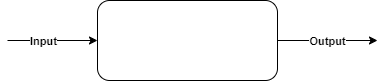
\includegraphics{figures/general_algorithm_diagram.png}
	\caption{Mô hình thuật toán chung, khối hình chữ nhật đen chưa định nghĩa gì, tượng trưng cho một chiếc hộp đen (blackbox). Hiểu rằng, thuật toán là biến đầu vào (Input) thành đầu ra (Output) tương ứng.}
	\label{fig:algorithm_architect_general}
\end{figure}

Như vậy khi tiến hành nêu ra định nghĩa thuật toán ở trên, ta nắm được một số thông tin mà sẽ được dùng để áp dụng kết nối chủ thể như "\textbf{hướng dẫn cho máy tính}", "\textbf{giải quyết vấn đề/bài toán}"

